\documentclass[8pt, xcolor=table,aspectratio=169]{beamer}



\usepackage[utf8]{inputenc}
\usepackage[T1]{fontenc}

\usepackage{helvet}
\usepackage{comment}
\usepackage{bm}

\usefonttheme[onlymath]{serif}

\usepackage{setspace}
\usepackage{tikz}
\usepackage{subcaption}
\usetikzlibrary{math}
\usetikzlibrary{calc}
\usetikzlibrary{arrows.meta}
\usetikzlibrary{positioning, fit, shapes.geometric, calc}
\usetikzlibrary{decorations.pathreplacing}

\usepackage{adjustbox}

\usepackage{pgfplots}
\pgfplotsset{compat=newest}
\pgfplotsset{every axis/.append style={
      label style={font=\small},
      tick label style={font=\small},
      legend style={font=\small\sf, row sep=-2pt},
      legend cell align={left}
    }
}

\def\centerarc[#1](#2)(#3:#4:#5)% Syntax: [draw options] (center) (initial angle:final angle:radius)
{ \draw[#1] ($(#2)+({#5*cos(#3)},{#5*sin(#3)})$) arc (#3:#4:#5); }

%\usepgfplotslibrary{external}
%\tikzexternalize[prefix=./fig/]
%\tikzexternalenable

\usepackage{amsmath,amssymb,amsfonts,amsthm}
\usepackage{mathtools}

\usepackage[absolute,showboxes,overlay]{textpos} %showboxes,overlay
\TPshowboxestrue            % affiche le contour des textblocks
\TPshowboxesfalse           % fait disparaitre le contour des textblocks
\textblockorigin{2mm}{8mm}  % origine des positions pour placer les textblocks

\usepackage{xcolor,colortbl,color}
\usepackage{framed}
\usepackage{mdframed}

\newtheorem{proposition}{Proposition}[theorem]

\mathtoolsset{showonlyrefs}

\usepackage{graphics}
\usepackage[pdf]{pstricks}
\usepackage{graphicx}
\usepackage{pstricks-add}
\usepackage{pst-node}
\usepackage{pst-plot}
\usepackage{pst-math}
\usepackage{pst-coil}
\usepackage{pst-grad}

% For checking draft
\usepackage{ifdraft}
% Backup slide numbers
\usepackage{appendixnumberbeamer}

% Box
\usepackage{tcolorbox}
\tcbuselibrary{skins, breakable}

%Algorithm
%\usepackage[lined,boxed]{algorithm2e}
\usepackage[boxed]{algorithm2e}
%Multirow
\usepackage{multirow}

%Itemize space
\usepackage{enumitem}
%\setlist[itemize]{label=\textbullet}
\setlist[itemize,1]{label=\scalebox{1.5}{\textbullet}}  % 1.5 = 150% de taille
%\setlist[itemize,2]{label=\scalebox{1.2}{\textbullet}}  % 1.5 = 150% de taille
\setlist[itemize,2]{label=\scalebox{1.2}{\(\circ\)}}
\usepackage{listings}

%----------------------------------------------------
% Colors
%----------------------------------------------------

\definecolor{colorField}{rgb}{0.2,0.6,0.2}
\definecolor{colorNumTra}{rgb}{1,0.5,0}
% \definecolor{colorOp}{rgb}{1,0.1,0.1}

\definecolor{darkrose}{rgb}{0.7,0,0.4}
\definecolor{darkblue}{rgb}{0.2,0.2,0.7}
\definecolor{darkorange}{rgb}{0.85,0.3,0.03}

\definecolor{main}{rgb}{0.25,0.35,0.55}
\definecolor{colorStruct}{rgb}{0.15,0.15,0.45}
%\definecolor{main}{rgb}{0.25,0.35,0.55}
%\definecolor{colorStruct}{rgb}{0.2,0.3,0.5}
\definecolor{colorStructLight}{rgb}{0.1,0.2,0.5}

\definecolor{lightlightlightgray}{rgb}{0.93,0.93,0.93}
\definecolor{lightlightgray}{rgb}{0.8,0.8,0.8}
\definecolor{lightgray}{rgb}{0.6,0.6,0.6}
\definecolor{darkgray}{rgb}{0.4,0.4,0.4}
\definecolor{darkdarkgray}{rgb}{0.2,0.2,0.2}

\definecolor{ubuntuorange}{rgb}{1,0.388235294,0.035294118}
\definecolor{ubuntuyellow}{rgb}{1,0.709803922,0.082352941}
\definecolor{ubuntured}{rgb}{0.788235294,0,0.08627451}
\definecolor{lightred}{rgb}{1,0.8,0.8}
\definecolor{lightred}{rgb}{1,0.85,0.7}
\definecolor{darkgreen}{rgb}{0.1,0.5,0.1}
\definecolor{ulggreen}{rgb}{0,0.286274509803922,0.309803921568627}
\definecolor{lightgreen}{rgb}{0.85,0.9,0.85}
\definecolor{lightyellow}{rgb}{1,0.8,0.5}
\definecolor{lightlightyellow}{rgb}{1,0.95,0.7}
\definecolor{bordeaux}{rgb}{0.686274509803922,0.149019607843137,0.149019607843137}
\definecolor{mainTOC}{rgb}{0.788235294,0,0.08627451}
\definecolor{myTeal}{HTML}{008080}
\definecolor{myReddish}{HTML}{d40000}
\definecolor{myGold}{HTML}{d4aa00}

%Used in GPU arch figure
\definecolor{gpumemorycolor}{HTML}{9013FE}
\definecolor{sharedmemorycolor}{HTML}{9B9B9B}

%%%%%%%%%%%%%%%%%%%%%%%%%%%%%%%%%%%%%%%%%%%%%%%%%%%%%%%%%%
\colorlet{colorTrans}{myReddish}
\colorlet{colorVol}{myTeal}
\colorlet{colorOp}{myGold}

\definecolor{lightblue}{rgb}{0.9,0.95,0.98}

%----------------------------------------------------
% Beamer
%----------------------------------------------------

\beamertemplatenavigationsymbolsempty
\setbeamercolor{frametitle}{fg=white,bg=colorStruct}

\newcommand{\axelfootline}{\begin{flushright}{\color{darkgray}\small\insertframenumber/\inserttotalframenumber}\;\;\;\;\end{flushright}}
\setbeamertemplate{footline}{\axelfootline}
\setbeamercolor{button}{bg=main,fg=white}
\setbeamertemplate{itemize items}[bullet]
\setbeamercolor{itemize item}{fg=main}
\setbeamertemplate{itemize subitem}[circle]
\setbeamercolor{itemize subitem}{fg=main}
\setbeamertemplate{itemize/enumerate body begin}{\normalsize}
\setbeamertemplate{itemize/enumerate subbody begin}{\normalsize}
\setbeamerfont{item}{size=\normalsize}
\setbeamerfont{subitem}{size=\normalsize}
\def\myframetitle#1#2{\frametitle{#2 \hspace{0pt plus 1 filll} {\small\color{yellow}[\:#1\:]\!\!\!} }}

\setbeamercolor{block title}{fg=white,bg=colorStruct!70!white}
\setbeamerfont{block title}{size=\normalsize}
\setbeamercolor{block body}{fg=black,bg=lightlightlightgray}
\setbeamertemplate{blocks}[shadow=false]
%\setbeamertemplate{blocks}[rounded][shadow=true]

\setbeamertemplate{itemize items}[circle]
\setbeamertemplate{itemize subitem}{$\circ$}

% ---------
% Symbols
% ---------

% Scalar valued versions
\newcommand{\matalg}[1]{\mathsf{#1}}
\newcommand{\vecalg}[1]{\mathsf{#1}}

% Vector valued versions
\newcommand{\matalgvv}[1]{\mathbf{\mathsf{#1}}}
\newcommand{\vecalgvv}[1]{\mathbf{\mathsf{#1}}}


\newcommand{\prodV}[2]{({\textstyle{#1}},{\textstyle{#2}})}
\newcommand{\prodS}[2]{\langle{\textstyle{#1}},{\textstyle{#2}}\rangle}

\newcommand{\PPs}{\mathbb{P}}
\newcommand{\PPv}{\pmb{\mathbb{P}}}

%% Miscellaneous
\renewcommand{\Re}{\operatorname{Re}}
\renewcommand{\Im}{\operatorname{Im}}

\newcommand{\im}{\imath}
\renewcommand{\i}{\im}

%% Differential operator
\newcommand{\grad}{\boldsymbol \nabla}
\renewcommand{\div}{\grad \cdot}
\newcommand{\curl}{\grad \times}

%% Bold uppercases
\newcommand{\BA}{\mathbf{A}}
\newcommand{\BB}{\mathbf{B}}
\newcommand{\BC}{\mathbf{C}}
\newcommand{\BD}{\mathbf{D}}
\newcommand{\BE}{\mathbf{E}}
\newcommand{\BF}{\mathbf{F}}
\newcommand{\BG}{\mathbf{G}}
\newcommand{\BH}{\mathbf{H}}
\newcommand{\BI}{\mathbf{I}}
\newcommand{\BJ}{\mathbf{J}}
\newcommand{\BK}{\mathbf{K}}
\newcommand{\BL}{\mathbf{L}}
\newcommand{\BM}{\mathbf{M}}
\newcommand{\BN}{\mathbf{N}}
\newcommand{\BO}{\mathbf{O}}
\newcommand{\BP}{\mathbf{P}}
\newcommand{\BQ}{\mathbf{Q}}
\newcommand{\BR}{\mathbf{R}}
\newcommand{\BS}{\mathbf{S}}
\newcommand{\BT}{\mathbf{T}}
\newcommand{\BU}{\mathbf{U}}
\newcommand{\BV}{\mathbf{V}}
\newcommand{\BW}{\mathbf{W}}
\newcommand{\BX}{\mathbf{X}}
\newcommand{\BY}{\mathbf{Y}}
\newcommand{\BZ}{\mathbf{Z}}

%% Bold lowercases
\newcommand{\vectort}[1]{\bm{#1}}
\newcommand{\ba}{\vectort{a}}
\newcommand{\bb}{\vectort{b}}
\newcommand{\bc}{\vectort{c}}
\newcommand{\bd}{\vectort{d}}
\newcommand{\be}{\vectort{e}}
\renewcommand{\bf}{\vectort{f}}
\newcommand{\bg}{\vectort{g}}
\newcommand{\bh}{\vectort{h}}
\newcommand{\bi}{\vectort{i}}
\newcommand{\bj}{\vectort{j}}
\newcommand{\bk}{\vectort{k}}
\newcommand{\bl}{\vectort{l}}
\newcommand{\bbm}{\vectort{m}} % avoid collision with bm
\newcommand{\bn}{\vectort{n}}
\newcommand{\bo}{\vectort{o}}
\newcommand{\bp}{\vectort{p}}
\newcommand{\bq}{\vectort{q}}
\newcommand{\br}{\vectort{r}}
\newcommand{\bs}{\vectort{s}}
\newcommand{\bt}{\vectort{t}}
\newcommand{\bu}{\vectort{u}}
\newcommand{\bv}{\vectort{v}}
\newcommand{\bw}{\vectort{w}}
\newcommand{\bx}{\vectort{x}}
\newcommand{\by}{\vectort{y}}
\newcommand{\bz}{\vectort{z}}
\newcommand{\bzero}{\mathbf{0}}
\newcommand{\bphi}{\boldsymbol{\phi}}

%% Curly uppercases
\newcommand{\CA}{\mathcal{A}}
\newcommand{\CB}{\mathcal{B}}
\newcommand{\CC}{\mathcal{C}}
\newcommand{\CD}{\mathcal{D}}
\newcommand{\CE}{\mathcal{E}}
\newcommand{\CF}{\mathcal{F}}
\newcommand{\CG}{\mathcal{G}}
\newcommand{\CH}{\mathcal{H}}
\newcommand{\CI}{\mathcal{I}}
\newcommand{\CJ}{\mathcal{J}}
\newcommand{\CK}{\mathcal{K}}
\newcommand{\CL}{\mathcal{L}}
\newcommand{\CM}{\mathcal{M}}
\newcommand{\CN}{\mathcal{N}}
\newcommand{\CO}{\mathcal{O}}
\newcommand{\CP}{\mathcal{P}}
\newcommand{\CQ}{\mathcal{Q}}
\newcommand{\CR}{\mathcal{R}}
\newcommand{\CS}{\mathcal{S}}
\newcommand{\CT}{\mathcal{T}}
\newcommand{\CU}{\mathcal{U}}
\newcommand{\CV}{\mathcal{V}}
\newcommand{\CW}{\mathcal{W}}
\newcommand{\CX}{\mathcal{X}}
\newcommand{\CY}{\mathcal{Y}}
\newcommand{\CZ}{\mathcal{Z}}

%% Caligraphic uppercases
\newcommand{\LA}{\mathscr{A}}
\newcommand{\LB}{\mathscr{B}}
\newcommand{\LC}{\mathscr{C}}
\newcommand{\LD}{\mathscr{D}}
\newcommand{\LE}{\mathscr{E}}
\newcommand{\LF}{\mathscr{F}}
\newcommand{\LG}{\mathscr{G}}
\newcommand{\LH}{\mathscr{H}}
\newcommand{\LI}{\mathscr{I}}
\newcommand{\LJ}{\mathscr{J}}
\newcommand{\LK}{\mathscr{K}}
\newcommand{\LL}{\mathscr{L}}
\newcommand{\LM}{\mathscr{M}}
\newcommand{\LN}{\mathscr{N}}
\newcommand{\LO}{\mathscr{O}}
\newcommand{\LP}{\mathscr{P}}
\newcommand{\LQ}{\mathscr{Q}}
\newcommand{\LR}{\mathscr{R}}
\newcommand{\LS}{\mathscr{S}}
\newcommand{\LT}{\mathscr{T}}
\newcommand{\LU}{\mathscr{U}}
\newcommand{\LV}{\mathscr{V}}
\newcommand{\LW}{\mathscr{W}}
\newcommand{\LX}{\mathscr{X}}
\newcommand{\LY}{\mathscr{Y}}
\newcommand{\LZ}{\mathscr{Z}}

%% Caligraphic uppercases
\newcommand{\tp}{\textup{\textrm{p}}}
\newcommand{\TA}{\textup{\textrm{A}}}
\newcommand{\TB}{\textup{\textrm{B}}}
\newcommand{\TC}{\textup{\textrm{C}}}
\newcommand{\TD}{\textup{\textrm{D}}}
\newcommand{\TE}{\textup{\textrm{E}}}
\newcommand{\TF}{\textup{\textrm{F}}}
\newcommand{\TG}{\textup{\textrm{G}}}
%\newcommand{\TH}{\textup{\textrm{H}}}
\newcommand{\TI}{\textup{\textrm{I}}}
\newcommand{\TJ}{\textup{\textrm{J}}}
\newcommand{\TK}{\textup{\textrm{K}}}
\newcommand{\TL}{\textup{\textrm{L}}}
\newcommand{\TM}{\textup{\textrm{M}}}
\newcommand{\TN}{\textup{\textrm{N}}}
\newcommand{\TO}{\textup{\textrm{O}}}
\newcommand{\TP}{\textup{\textrm{P}}}
\newcommand{\TQ}{\textup{\textrm{Q}}}
\newcommand{\TR}{\textup{\textrm{R}}}
\newcommand{\TS}{\textup{\textrm{S}}}
\newcommand{\TT}{\textup{\textrm{T}}}
\newcommand{\TU}{\textup{\textrm{U}}}
\newcommand{\TV}{\textup{\textrm{V}}}
\newcommand{\TW}{\textup{\textrm{W}}}
\newcommand{\TX}{\textup{\textrm{X}}}
\newcommand{\TY}{\textup{\textrm{Y}}}
\newcommand{\TZ}{\textup{\textrm{Z}}}

%% Bold curly uppercases
\newcommand{\BCA}{\boldsymbol{\CA}}
\newcommand{\BCB}{\boldsymbol{\CB}}
\newcommand{\BCC}{\boldsymbol{\CC}}
\newcommand{\BCD}{\boldsymbol{\CD}}
\newcommand{\BCE}{\boldsymbol{\CE}}
\newcommand{\BCF}{\boldsymbol{\CF}}
\newcommand{\BCG}{\boldsymbol{\CG}}
\newcommand{\BCH}{\boldsymbol{\CH}}
\newcommand{\BCI}{\boldsymbol{\CI}}
\newcommand{\BCJ}{\boldsymbol{\CJ}}
\newcommand{\BCK}{\boldsymbol{\CK}}
\newcommand{\BCL}{\boldsymbol{\CL}}
\newcommand{\BCM}{\boldsymbol{\CM}}
\newcommand{\BCN}{\boldsymbol{\CN}}
\newcommand{\BCO}{\boldsymbol{\CO}}
\newcommand{\BCP}{\boldsymbol{\CP}}
\newcommand{\BCQ}{\boldsymbol{\CQ}}
\newcommand{\BCR}{\boldsymbol{\CR}}
\newcommand{\BCS}{\boldsymbol{\CS}}
\newcommand{\BCT}{\boldsymbol{\CT}}
\newcommand{\BCU}{\boldsymbol{\CU}}
\newcommand{\BCV}{\boldsymbol{\CV}}
\newcommand{\BCW}{\boldsymbol{\CW}}
\newcommand{\BCX}{\boldsymbol{\CX}}
\newcommand{\BCY}{\boldsymbol{\CY}}
\newcommand{\BCZ}{\boldsymbol{\CZ}}

%% Bold caligraphic uppercases
\newcommand{\BLA}{\pmb{\LA}}
\newcommand{\BLB}{\pmb{\LB}}
\newcommand{\BLC}{\pmb{\LC}}
\newcommand{\BLD}{\pmb{\LD}}
\newcommand{\BLE}{\pmb{\LE}}
\newcommand{\BLF}{\pmb{\LF}}
\newcommand{\BLG}{\pmb{\LG}}
\newcommand{\BLH}{\pmb{\LH}}
\newcommand{\BLI}{\pmb{\LI}}
\newcommand{\BLJ}{\pmb{\LJ}}
\newcommand{\BLK}{\pmb{\LK}}
\newcommand{\BLL}{\pmb{\LL}}
\newcommand{\BLM}{\pmb{\LM}}
\newcommand{\BLN}{\pmb{\LN}}
\newcommand{\BLO}{\pmb{\LO}}
\newcommand{\BLP}{\pmb{\LP}}
\newcommand{\BLQ}{\pmb{\LQ}}
\newcommand{\BLR}{\pmb{\LR}}
\newcommand{\BLS}{\pmb{\LS}}
\newcommand{\BLT}{\pmb{\LT}}
\newcommand{\BLU}{\pmb{\LU}}
\newcommand{\BLV}{\pmb{\LV}}
\newcommand{\BLW}{\pmb{\LW}}
\newcommand{\BLX}{\pmb{\LX}}
\newcommand{\BLY}{\pmb{\LY}}
\newcommand{\BLZ}{\pmb{\LZ}}

%% Bold text-up
\newcommand{\BTA}{\pmb{\TA}}
\newcommand{\BTB}{\pmb{\TB}}
\newcommand{\BTC}{\pmb{\TC}}
\newcommand{\BTD}{\pmb{\TD}}
\newcommand{\BTE}{\pmb{\TE}}
\newcommand{\BTF}{\pmb{\TF}}
\newcommand{\BTG}{\pmb{\TG}}
%\newcommand{\BTH}{\pmb{\TH}}
\newcommand{\BTI}{\pmb{\TI}}
\newcommand{\BTJ}{\pmb{\TJ}}
\newcommand{\BTK}{\pmb{\TK}}
\newcommand{\BTL}{\pmb{\TL}}
\newcommand{\BTM}{\pmb{\TM}}
\newcommand{\BTN}{\pmb{\TN}}
\newcommand{\BTO}{\pmb{\TO}}
\newcommand{\BTP}{\pmb{\TP}}
\newcommand{\BTQ}{\pmb{\TQ}}
\newcommand{\BTR}{\pmb{\TR}}
\newcommand{\BTS}{\pmb{\TS}}
\newcommand{\BTT}{\pmb{\TT}}
\newcommand{\BTU}{\pmb{\TU}}
\newcommand{\BTV}{\pmb{\TV}}
\newcommand{\BTW}{\pmb{\TW}}
\newcommand{\BTX}{\pmb{\TX}}
\newcommand{\BTY}{\pmb{\TY}}
\newcommand{\BTZ}{\pmb{\TZ}}

%% Matlab style
\newcommand{\MA}{\matalg{A}}
\newcommand{\MB}{\matalg{B}}
\newcommand{\MC}{\matalg{C}}
\newcommand{\MD}{\matalg{D}}
\newcommand{\ME}{\matalg{E}}
\newcommand{\MF}{\matalg{F}}
\newcommand{\MG}{\matalg{G}}
\newcommand{\MH}{\matalg{H}}
\newcommand{\MI}{\matalg{I}}
\newcommand{\MJ}{\matalg{J}}
\newcommand{\MK}{\matalg{K}}
\newcommand{\ML}{\matalg{L}}
\newcommand{\MM}{\matalg{M}}
\newcommand{\MN}{\matalg{N}}
\newcommand{\MO}{\matalg{O}}
\newcommand{\MP}{\matalg{P}}
\newcommand{\MQ}{\matalg{Q}}
\newcommand{\MR}{\matalg{R}}
\newcommand{\MS}{\matalg{S}}
\newcommand{\MT}{\matalg{T}}
\newcommand{\MU}{\matalg{U}}
\newcommand{\MV}{\matalg{V}}
\newcommand{\MW}{\matalg{W}}
\newcommand{\MX}{\matalg{X}}
\newcommand{\MY}{\matalg{Y}}
\newcommand{\MZ}{\matalg{Z}}
\newcommand{\MPi}{\matalg{\Pi}}

% \newcommand{\ma}{\matalg{a}}
\newcommand{\mb}{\matalg{b}}
\newcommand{\mc}{\matalg{c}}
\newcommand{\md}{\matalg{d}}
\newcommand{\me}{\matalg{e}}
\newcommand{\mf}{\matalg{f}}
\newcommand{\mg}{\matalg{g}}
\newcommand{\mh}{\matalg{h}}
% \newcommand{\mi}{\matalg{i}}
% \newcommand{\mj}{\matalg{j}}
% \newcommand{\mk}{\matalg{k}}
% \newcommand{\ml}{\matalg{l}}
% \newcommand{\mm}{\matalg{m}}
% \newcommand{\mn}{\matalg{n}}
% \newcommand{\mo}{\matalg{o}}
\newcommand{\mmp}{\matalg{p}}
\newcommand{\mq}{\matalg{q}}
\newcommand{\mr}{\matalg{r}}
\newcommand{\ms}{\matalg{s}}
\newcommand{\mt}{\matalg{t}}
%\newcommand{\mu}{\matalg{u}}
\newcommand{\mv}{\matalg{v}}
\newcommand{\mw}{\matalg{w}}
\newcommand{\mx}{\matalg{x}}
\newcommand{\my}{\matalg{y}}
\newcommand{\mz}{\matalg{z}}

% Greek
\newcommand{\bpi}{\boldsymbol{\pi}}
\newcommand{\bmu}{\boldsymbol{\mu}}
\newcommand{\bvepsilon}{\boldsymbol{\varepsilon}}
\newcommand{\bxi}{\boldsymbol{\xi}}
\newcommand{\bgamma}{\mathsf{\gamma}}
\newcommand{\BPi}{\mathbf{\Pi}}
\newcommand{\BTPi}{\mathbf{\mathsf{\Pi}}}

% rmsub
\newcommand{\rmsub}[1]{_{\mathrm{#1}}}
\newcommand{\rmsup}[1]{^{\mathrm{#1}}}

\newcommand{\mycolorbar}[3]{%
  \begin{tikzpicture}[rotate=0]
		\begin{axis}[
			hide axis,
			scale only axis,
			height=0pt,
			width=0pt,
			colormap/jet,
			colorbar horizontal,
			point meta min=#1,
			point meta max=#2,
			colorbar style={
				width=#3\linewidth,
				height=2mm,
				rotate=0,
				title=,
				xtick={#1,#2},
				xtick style={draw=none},
				axis line style={draw=none},
				xticklabel style={xshift=0pt,yshift=0pt},
				title style={xshift=2.5cm,yshift=3.2cm},
				%xmode=auto,
			}
			]
		\end{axis}
  \end{tikzpicture}%
}
\newcommand{\surface}[1]{\textcolor{colorTrans}{#1}}
\newcommand{\volume}[1]{\textcolor{myTeal}{#1}}
\definecolor{pythonorange}{RGB}{255,127,0}
\definecolor{pythongreen}{RGB}{0,153,0}
\definecolor{pythonblue}{RGB}{0,0,180}
\captionsetup[figure]{labelformat=empty}

\newif\ifbackup
\backupfalse

\newif\ifDGslide
\DGslidetrue

\setbeamertemplate{section in toc}[sections numbered]
%% Initialize a custom counter for tracking the section numbers

% Customize the table of contents spacing
%\setbeamertemplate{section in toc}[] % Remove numbers and add ball for sections
%\setbeamertemplate{subsection in toc}[default] % Default style for subsections

% Adjust spacing between sections and subsections
\setlength{\leftskip}{0pt} % Set left margin for TOC
\setlength{\rightskip}{0pt} % Set right margin for TOC
\setlength{\parskip}{2mm} % Space between paragraphs in TOC (sections and subsections)

% Define colors for active and inactive sections
\definecolor{activecolor}{rgb}{1,1,0} % yellow
\definecolor{inactivecolor}{rgb}{0.6, 0.6, 0.6} % equivalent to black!40

\setbeamertemplate{section in toc shaded}[default][100]

% Use \AtBeginSection to customize the TOC slide
\AtBeginSection[]{
    % Change the background color for the TOC slide
    \setbeamercolor{background canvas}{bg=colorStruct} % Set TOC background color
    \setbeamertemplate{footline}{} % Suppress footline (including frame number)
    \begin{frame}[noframenumbering]
      \frametitle{Outline}
      \setbeamercolor{section in toc shaded}{fg=inactivecolor} % Inactive color for shaded sections
      \setbeamercolor{section in toc}{fg=activecolor} % Active color for current section
      \tableofcontents[currentsection, hideothersubsections] % Show current section with hidden subsections
    \end{frame}
    \setbeamertemplate{footline}{\axelfootline} % Reset the footline
    % Reset colors to default after TOC slide
    \setbeamercolor{background canvas}{bg=} % Reset background color
    \setbeamercolor{section in toc}{fg=black} % Reset TOC section color to default
    \setbeamercolor{subsection in toc}{fg=black} % Reset TOC subsection color to default
}

\newcommand{\fluxfigure}{
       \begin{tikzpicture}[xscale=1,yscale=1]
        %\filldraw[color=black, fill=black!10, thick] (0,0) ellipse (1.3 and 0.6);
        \draw[fill=black!5,thick] (0,0) -- (1,0) -- (1.5,0.7) -- (0.5,0.7) -- cycle;
        \draw[thick] (0.5,0.7) -- (1,0);
        \draw[-latex, color=black, thick] (0.6,0.55) -- (0.95,0.80);
        %\draw (0.70,0.12) node {\color{black!50}\footnotesize$K$};
        %\draw (1.03,0.3) node {\color{black!50}\footnotesize$K'$};
        \draw (0.95,0.9) node {\color{black}\scriptsize$\mathbf{n}_{K,F}$};
        \draw (0.70,0.2) node {\scriptsize$F$};
        \draw (0.35,0.15) node {\color{black!75}\footnotesize$K$};
        \draw (1.16,0.53) node {\color{black!75}\footnotesize$K'$};
        \draw[-latex, color=black, thick] (0.80,-0.45) -- (1.50, 0.05);
        \draw[latex-, color=colorTrans, thick] (0.90,-0.65) -- (1.60,-0.15);
        \draw (1.85, 0.17) node {\color{black}$\scriptsize g_{K,F}^{\oplus}$};
        \draw (2.05,-0.75) node
          {\color{colorTrans}$\scriptsize g_{K,F}^{\ominus}\color{black}\ \ (=g_{K',F}^{\oplus})$};
      \end{tikzpicture}
    }

\begin{document}

%%%%%%%%%%%%%%%%%%%%%%%%%%%%%%%%%%%%%%%%%%%%%%%%%%%%%%%%%%%%%%%%%%%%%%%%%%%%%%%%

{\setbeamertemplate{footline}{}
\frame[noframenumbering]{


  \begin{textblock*}{160mm}(-2mm,30mm)
    \textblockcolor{colorStruct}
    \begin{center}
      \vspace{1mm}
      {\LARGE\color{white}{High-order Lagrange elements in  \texttt{FreeFem++}}   
}
      \vspace{1mm}
    \end{center}
  \end{textblock*}

  \begin{textblock*}{160mm}(-2mm,50mm)
    \textblockcolor{}
    \centering
    {\large \underline{\textsc{A. Chabib}}, \textsc{P-H. Tournier}, \textsc{F. Hecht} } \\ \vspace{0.5mm}
    \textcolor{black!50}{{Laboratoire Jacques-Louis Lions }} \\
    \textcolor{black!50}{{CNRS, Sorbonne Université UPMC , France}}\\
    \textcolor{black!50}{{ALPINES team, Centre Inria de Paris}}

  \end{textblock*}

  \begin{textblock*}{160mm}(-2mm,60mm)
    \textblockcolor{}
  
  \end{textblock*}
  \vspace{1cm}
  \begin{textblock*}{160mm}(-2mm,63mm)
    \textblockcolor{}
    \begin{center}
      %\small
      {\large\texttt{FreeFem} Days}\\
      December 17, 2025

    \end{center}
  \end{textblock*}



  \begin{textblock*}{150mm}(25mm,2mm)
    \textblockcolor{}
    \includegraphics[height=16mm]{figures/logos/ljll.png}
    \hspace{0.2cm}
    \includegraphics[height=16mm]{figures/logos/LOGO_CNRS_BLEU.png}
    \hspace{0.2cm}
    \includegraphics[height=15mm]{figures/logos/LOGO_SorbonneU_0.jpg}
    \hspace{0.1cm}
    \includegraphics[height=15mm]{figures/logos/inr_logo_noir.png}
    \hspace{0.2cm}

  \end{textblock*}
  %\begin{textblock*}{117mm}(4mm,100mm)
  %  \textblockcolor{}
  %  \hfill
  %  %\includegraphics[width=25mm]{img/internoise2024.png}
  %\end{textblock*}


%   \begin{textblock*}{150mm}(35mm,58mm)
%     \textblockcolor{}
    
%     \includegraphics[height=18mm]{figures/logos/LOGO_CNRS_BLEU.png}
%     %\hspace{2mm}    
%     %\includegraphics[height=6mm]{figures/logos/logoENSTA.png}
%     %\hspace{2mm}
%     %\includegraphics[height=10mm]{figures/logos/logoIPParis.png}
%   \end{textblock*}
  % \begin{textblock*}{150mm}(0mm,35mm)
  %   \textblockcolor{}
  %   \includegraphics[height=15mm]{figures/logos/labelANR.png}
  % \end{textblock*}
%   \begin{textblock*}{150mm}(55mm,62mm)
%     \textblockcolor{}
%     %\includegraphics[height=8mm]{figures/logos/logoENSTA.png}
%     \includegraphics[height=20mm]{figures/logos/ljll.png}
  
% \end{textblock*}

}}

%%%%%%%%%%%%%%%%%%%%%%%%%%%%%%%%%%%%%%%%%%%%%%%%%%%%%%%%%%%%%%%%%%%%%%%%%%%%%%%%
\begin{frame}{Motivation}
    \begin{center}
    \textbf{Finite element} solution of \textbf{time-harmonic wave propagation problems}
  \end{center}

    \fcolorbox{black}{black!7}{\begin{minipage}{50mm}
        \centering
        \vspace{3mm}
        \textbf{\color{colorStruct}Helmholtz problem:} \\ \vspace{3mm}
        $
          \left\{\;
          \begin{aligned}
             & -\Delta {\color{colorVol}p} - \omega^2 {\color{colorVol}p} = s
             &
             & \text{in $\Omega$}
            \\
             & \text{Boundary conditions}
             &
             & \text{on $\partial\Omega$}
          \end{aligned}
          \right.
        % $ \\ \vspace{3mm}
        % $
        %   \Rightarrow
        %   \quad
        %   \fbox{\hspace{1mm}$\mathbf{\matalg{A}{\color{colorVol}\vecalg{x}} = \vecalg{b}}$\hspace{1mm}}
        $
        \vspace{3mm}
        
        \textbf{{\color{colorStruct}Finite element error:}}
        \vspace{3mm}

        %$ \lVert {\color{colorVol}p} - {\color{colorVol}p_h}\lVert  _{H^1} \leq C_1(\omega h)^k + C_2\omega^{(k+1)}h^k$
        $ \lVert {\color{colorVol}p} - {\color{colorVol}p_h}\lVert  _{H^1} \leq C_\omega h^k\lVert {\color{colorVol}p}\lVert_{H^{k+1}}$

      \end{minipage}}
    \hfill
    \begin{minipage}{35mm}
      \begin{center}
        {\small\color{black!50} Finite element mesh} \vspace{1mm}

        \includegraphics[height=30mm]{figures/intro/turbofan_mesh.png}
      \end{center}
    \end{minipage}
    \hfill
    \begin{minipage}{35mm}
      \begin{center}
        {\small\color{black!50} Numerical field} \vspace{1mm}

        \includegraphics[height=30mm]{figures/intro/turbofan_a2500.png}
      \end{center}
    \end{minipage}
 %\vspace{3mm}

  {
    %\small
    \begin{align}
      \begin{aligned}
        % & \text{Complicated material coefficients $\bmu, \bvepsilon$}
        %\\
         & \text{High frequency {\small(large $\omega$)}}
        \\
         & \text{Phenomena close to resonance}
        \\
        % & \text{Good accuracy}
      \end{aligned}
      \ \ \ \leadsto
      \left\{\ \begin{aligned}
                  & \text{Fine mesh {\small(small $h$)}} \quad \uncover<2>{\textcolor{blue}{\large \checkmark}}
                 \\
                  & \text{High-order basis functions {\small(large $k$)}} \quad \uncover<2>{\textcolor{red}{{\text{X Limited to } P_4} }  }
                 %\\
                  %& \text{Large unstructured sparse system / Many DOFs}
                 %\\
                  %& \textbf{\color{ubuntured}Standard direct/iterative solvers are slow}
               \end{aligned}\right.
    \end{align}
  }

% Dans le cadre de la méthode des éléments finis appliquée, par exemple, à l’équation
%  d’onde de type Helmholtz, l’erreur numérique peut se dégrader de manière significative.
%   Cette détérioration est bien décrite par une inégalité classique qui sépare l’erreur 
%   totale en deux contributions :
% 1-l’erreur d’approximation, liée à la capacité de l’espace discret à représenter la 
% solution exacte, 
% 2-l’erreur de pollution, spécifique aux problèmes oscillatoires et qui 
% augmente avec le nombre d’ondes résolues.
% Pour atténuer cette erreur, une première approche consiste à raffiner le maillage. 
% Bien que ce procédé soit efficace, il peut devenir extrêmement coûteux en termes de 
% mémoire et de temps de calcul, car le raffinement doit compenser la croissance de 
% l’erreur de pollution, qui croît généralement avec un facteur en kh ou k^2h, où k est 
% le nombre d’onde.
% Une alternative plus performante consiste à augmenter l’ordre d’interpolation, 
% c’est-à-dire à utiliser des éléments finis d’ordre élevé (augmentation du paramètre p). 
% Cette stratégie est souvent plus efficace que le simple raffinement du maillage : elle 
% permet de mieux capturer l’oscillation de la solution avec beaucoup moins d’éléments, 
% réduit l’impact de l’erreur de pollution, et améliore la précision globale pour un coût 
% numérique comparable, voire inférieur. En pratique, les méthodes à ordre élevé 
% constituent donc une approche plus adaptée pour les problèmes oscillatoires de 
% type Helmholtz.
\end{frame}
%%%%%%%%%%%%%%%%%%%%%%%%%%%%%%%%%%%%%%%%%%%%%%%%%%%%%%%%%%%%%%%%%%%%%%%%%%%%%%%%
\begin{frame}{Lagrange FE in \texttt{FreeFem++} I}
  \vspace{0.5cm}
  \begin{minipage}{70mm}
 \verbatiminput{cpp_codes/Element_P4.cpp}
  \end{minipage}
\uncover<2>{
  \begin{tikzpicture}[remember picture, overlay]
      % Place the whole diagram 2cm from top-left
      \node at (current page.north west) [xshift=9.8cm, yshift=-2.5cm] {
          \begin{tikzpicture}
              \draw[color=blue][->, thick] (0,0) -- (1,0) ;
              \node at (1.7,0) {\textcolor{blue}{\# DOF =15}};
          \end{tikzpicture}
      };

      \node at (current page.north west) [xshift=6.8cm, yshift=-2.15cm] {
      \begin{tikzpicture}
          \draw[color=blue][->, thick] (0,0) -- (1,0) ;
          \node at (2.2,0) {\textcolor{blue}{Interpolation order}};
      \end{tikzpicture}
      };

      \node at (current page.north west) [xshift=6.6cm, yshift=-2.82cm] {
      \begin{tikzpicture}
          \draw[color=blue][->, thick] (0,0) -- (1,0) ;
          \node at (2.5,0) {\textcolor{blue}{Topological information}};
      \end{tikzpicture}
      };

      \node at (current page.north west) [xshift=9.2cm, yshift=-3.15cm] {
      \begin{tikzpicture}
          \draw[color=blue][->, thick] (0,0) -- (1,0) ;
          \node at (4.3,0) {\textcolor{blue}{Used to construct normal Not needed for Lagrange}};
      \end{tikzpicture}
      };

      \node at (current page.north west) [xshift=9.8cm, yshift=-3.85cm] {
      \begin{tikzpicture}
          \draw[decorate,color=blue, decoration={brace, amplitude=10pt, mirror}]
          (0,1) -- (0,1.8)  node[midway,right=3mm]{Shape functions: $\displaystyle \Phi _i =\overset{3}{\underset{j=0}{\Pi }} \frac{1}{\texttt{ff[i]}}
          \left (\lambda _{\texttt{nn[i][j]}}-\texttt{aa[i][j]}\right ) $ \texttt{.hpp}};
      \end{tikzpicture}
      };

      \node at (current page.north west) [xshift=7.7cm, yshift=-4.85cm] {
      \begin{tikzpicture}
          \draw[decorate,color=blue, decoration={brace, amplitude=10pt, mirror}]
          (0,1) -- (0,1.8)  node[midway,right=3mm]{Nodes barycentric coordinates \texttt{.hpp}};
      \end{tikzpicture}
      };

      \node at (current page.north west) [xshift=10.1cm, yshift=-5.8cm] {
      \begin{tikzpicture}
          \draw [color=blue, line width=0.5mm](0.4,0) rectangle (6.8,0.5);
          \node[right] at (7,0.25){\textcolor{blue}{Parent class constructor}};
        \end{tikzpicture}
      };
  \end{tikzpicture}

}
\end{frame}
%%%%%%%%%%%%%%%%%%%%%%%%%%%%%%%%%%%%%%%%%%%%%%%%%%%%%%%%%%%%%%%%%%%%%%%%%%%%%%%%
\begin{frame}{Lagrange FE in \texttt{FreeFem++} II}
  \VerbatimInput[firstline=14,lastline=14]{cpp_codes/Element_P4.cpp}
  \begin{center}
\begin{tabular}{ c c c }
 Argument & Value $P_4$ & Value $P_k$ \\ 
 \hline\\
 \# dof & \texttt{15} & $\displaystyle\frac{(k+1)(k+2)}{2}$ \\  
 Dimension FE & \texttt{1} & \texttt{1}  \\
 Array containing topological information & \texttt{Data} & \texttt{Data}  \\  
 Number of subdivisions for plotting  & \texttt{4} & $k$  \\  
 Number of sub-finite elements & \texttt{1} & \texttt{1}  \\  
 \# dof+ non-symmetric permutation of dofs on edges & \texttt{15+6} & \# dof+ $3\times ( (k \% 2) ? (k- 1) : (k - 2)) $  \\  
 Number of interpolation points & \texttt{15} & $\displaystyle\frac{(k+1)(k+2)}{2}$  \\  
 Normal components array  & \texttt{0} & \texttt{0}  \\  

\end{tabular}
\end{center}
% \begin{itemize}
  % \item 1: scalar function space(not vector field).
  % \item Data: Numbering and relationship between DOFs and nodes.
  % \item 4: To visualize the element, it's subdivided into $k$ sub-elements.
  % \item The 15 points where functions are evaluated to construct the interpolant.
% \end{itemize}
\end{frame}

%%%%%%%%%%%%%%%%%%%%%%%%%%%%%%%%%%%%%%%%%%%%%%%%%%%%%%%%%%%%%%%%%%%%%%%%%%%%%%%%
\begin{frame}{Lagrange FE in \texttt{FreeFem++} III}
\begin{minipage}{60mm}
          \begin{figure}
        
         \resizebox{\textwidth}{!}{%
    

\tikzset{every picture/.style={line width=0.75pt}} %set default line width to 0.75pt        

\begin{tikzpicture}[x=0.75pt,y=0.75pt,yscale=-1,xscale=1]
%uncomment if require: \path (0,442); %set diagram left start at 0, and has height of 442

%Shape: Right Triangle [id:dp4009669958873615] 
\draw   (42,36.5) -- (342,336.5) -- (42,336.5) -- cycle ;
%Shape: Circle [id:dp48544102153127466] 
\draw  [color={rgb, 255:red, 245; green, 166; blue, 35 }  ,draw opacity=1 ][fill={rgb, 255:red, 245; green, 166; blue, 35 }  ,fill opacity=1 ] (40,37) .. controls (40,35.62) and (41.12,34.5) .. (42.5,34.5) .. controls (43.88,34.5) and (45,35.62) .. (45,37) .. controls (45,38.38) and (43.88,39.5) .. (42.5,39.5) .. controls (41.12,39.5) and (40,38.38) .. (40,37) -- cycle ;
%Shape: Circle [id:dp23315037848017595] 
\draw  [color={rgb, 255:red, 245; green, 166; blue, 35 }  ,draw opacity=1 ][fill={rgb, 255:red, 245; green, 166; blue, 35 }  ,fill opacity=1 ] (40,337) .. controls (40,335.62) and (41.12,334.5) .. (42.5,334.5) .. controls (43.88,334.5) and (45,335.62) .. (45,337) .. controls (45,338.38) and (43.88,339.5) .. (42.5,339.5) .. controls (41.12,339.5) and (40,338.38) .. (40,337) -- cycle ;
%Shape: Circle [id:dp8936963841024985] 
\draw  [color={rgb, 255:red, 245; green, 166; blue, 35 }  ,draw opacity=1 ][fill={rgb, 255:red, 245; green, 166; blue, 35 }  ,fill opacity=1 ] (339,337) .. controls (339,335.62) and (340.12,334.5) .. (341.5,334.5) .. controls (342.88,334.5) and (344,335.62) .. (344,337) .. controls (344,338.38) and (342.88,339.5) .. (341.5,339.5) .. controls (340.12,339.5) and (339,338.38) .. (339,337) -- cycle ;
%Shape: Circle [id:dp5450874183983604] 
\draw  [color={rgb, 255:red, 245; green, 166; blue, 35 }  ,draw opacity=1 ][fill={rgb, 255:red, 245; green, 166; blue, 35 }  ,fill opacity=1 ] (115,337) .. controls (115,335.62) and (116.12,334.5) .. (117.5,334.5) .. controls (118.88,334.5) and (120,335.62) .. (120,337) .. controls (120,338.38) and (118.88,339.5) .. (117.5,339.5) .. controls (116.12,339.5) and (115,338.38) .. (115,337) -- cycle ;
%Shape: Circle [id:dp8950759974968507] 
\draw  [color={rgb, 255:red, 245; green, 166; blue, 35 }  ,draw opacity=1 ][fill={rgb, 255:red, 245; green, 166; blue, 35 }  ,fill opacity=1 ] (190,337) .. controls (190,335.62) and (191.12,334.5) .. (192.5,334.5) .. controls (193.88,334.5) and (195,335.62) .. (195,337) .. controls (195,338.38) and (193.88,339.5) .. (192.5,339.5) .. controls (191.12,339.5) and (190,338.38) .. (190,337) -- cycle ;
%Shape: Circle [id:dp6396385107320545] 
\draw  [color={rgb, 255:red, 245; green, 166; blue, 35 }  ,draw opacity=1 ][fill={rgb, 255:red, 245; green, 166; blue, 35 }  ,fill opacity=1 ] (265,337) .. controls (265,335.62) and (266.12,334.5) .. (267.5,334.5) .. controls (268.88,334.5) and (270,335.62) .. (270,337) .. controls (270,338.38) and (268.88,339.5) .. (267.5,339.5) .. controls (266.12,339.5) and (265,338.38) .. (265,337) -- cycle ;
%Shape: Circle [id:dp11681249861686172] 
\draw  [color={rgb, 255:red, 245; green, 166; blue, 35 }  ,draw opacity=1 ][fill={rgb, 255:red, 245; green, 166; blue, 35 }  ,fill opacity=1 ] (40,112) .. controls (40,110.62) and (41.12,109.5) .. (42.5,109.5) .. controls (43.88,109.5) and (45,110.62) .. (45,112) .. controls (45,113.38) and (43.88,114.5) .. (42.5,114.5) .. controls (41.12,114.5) and (40,113.38) .. (40,112) -- cycle ;
%Shape: Circle [id:dp0073784290505588546] 
\draw  [color={rgb, 255:red, 245; green, 166; blue, 35 }  ,draw opacity=1 ][fill={rgb, 255:red, 245; green, 166; blue, 35 }  ,fill opacity=1 ] (40,262) .. controls (40,260.62) and (41.12,259.5) .. (42.5,259.5) .. controls (43.88,259.5) and (45,260.62) .. (45,262) .. controls (45,263.38) and (43.88,264.5) .. (42.5,264.5) .. controls (41.12,264.5) and (40,263.38) .. (40,262) -- cycle ;
%Shape: Circle [id:dp3011150737603383] 
\draw  [color={rgb, 255:red, 245; green, 166; blue, 35 }  ,draw opacity=1 ][fill={rgb, 255:red, 245; green, 166; blue, 35 }  ,fill opacity=1 ] (40,187) .. controls (40,185.62) and (41.12,184.5) .. (42.5,184.5) .. controls (43.88,184.5) and (45,185.62) .. (45,187) .. controls (45,188.38) and (43.88,189.5) .. (42.5,189.5) .. controls (41.12,189.5) and (40,188.38) .. (40,187) -- cycle ;
%Shape: Circle [id:dp3527568040416259] 
\draw  [color={rgb, 255:red, 245; green, 166; blue, 35 }  ,draw opacity=1 ][fill={rgb, 255:red, 245; green, 166; blue, 35 }  ,fill opacity=1 ] (115.5,112) .. controls (115.5,110.62) and (116.62,109.5) .. (118,109.5) .. controls (119.38,109.5) and (120.5,110.62) .. (120.5,112) .. controls (120.5,113.38) and (119.38,114.5) .. (118,114.5) .. controls (116.62,114.5) and (115.5,113.38) .. (115.5,112) -- cycle ;
%Shape: Circle [id:dp1570657349346286] 
\draw  [color={rgb, 255:red, 245; green, 166; blue, 35 }  ,draw opacity=1 ][fill={rgb, 255:red, 245; green, 166; blue, 35 }  ,fill opacity=1 ] (115,187) .. controls (115,185.62) and (116.12,184.5) .. (117.5,184.5) .. controls (118.88,184.5) and (120,185.62) .. (120,187) .. controls (120,188.38) and (118.88,189.5) .. (117.5,189.5) .. controls (116.12,189.5) and (115,188.38) .. (115,187) -- cycle ;
%Shape: Circle [id:dp65670462147046] 
\draw  [color={rgb, 255:red, 245; green, 166; blue, 35 }  ,draw opacity=1 ][fill={rgb, 255:red, 245; green, 166; blue, 35 }  ,fill opacity=1 ] (190,187) .. controls (190,185.62) and (191.12,184.5) .. (192.5,184.5) .. controls (193.88,184.5) and (195,185.62) .. (195,187) .. controls (195,188.38) and (193.88,189.5) .. (192.5,189.5) .. controls (191.12,189.5) and (190,188.38) .. (190,187) -- cycle ;
%Shape: Circle [id:dp5366172166400391] 
\draw  [color={rgb, 255:red, 245; green, 166; blue, 35 }  ,draw opacity=1 ][fill={rgb, 255:red, 245; green, 166; blue, 35 }  ,fill opacity=1 ] (190,262) .. controls (190,260.62) and (191.12,259.5) .. (192.5,259.5) .. controls (193.88,259.5) and (195,260.62) .. (195,262) .. controls (195,263.38) and (193.88,264.5) .. (192.5,264.5) .. controls (191.12,264.5) and (190,263.38) .. (190,262) -- cycle ;
%Shape: Circle [id:dp6454133942358746] 
\draw  [color={rgb, 255:red, 245; green, 166; blue, 35 }  ,draw opacity=1 ][fill={rgb, 255:red, 245; green, 166; blue, 35 }  ,fill opacity=1 ] (265,262) .. controls (265,260.62) and (266.12,259.5) .. (267.5,259.5) .. controls (268.88,259.5) and (270,260.62) .. (270,262) .. controls (270,263.38) and (268.88,264.5) .. (267.5,264.5) .. controls (266.12,264.5) and (265,263.38) .. (265,262) -- cycle ;
%Straight Lines [id:da951267851143512] 
%\draw [line width=1.5]    (133.89,204.14) -- (149.81,218.2) -- (165.62,232.16) ;
%\draw [shift={(168.62,234.8)}, rotate = 221.44] [fill={rgb, 255:red, 0; green, 0; blue, 0 }  ][line width=0.08]  [draw opacity=0] (9.29,-4.46) -- (0,0) -- (9.29,4.46) -- cycle    ;
%Straight Lines [id:da3260676891247549] 
%\draw [line width=1.5]    (169.4,260.5) -- (155.01,260.57) -- (149.84,260.61) -- (133.42,260.77) ;
%\draw [shift={(129.42,260.8)}, rotate = 359.47] [fill={rgb, 255:red, 0; green, 0; blue, 0 }  ][line width=0.08]  [draw opacity=0] (9.29,-4.46) -- (0,0) -- (9.29,4.46) -- cycle    ;
%Shape: Circle [id:dp8416643705036926] 
\draw  [color={rgb, 255:red, 245; green, 166; blue, 35 }  ,draw opacity=1 ][fill={rgb, 255:red, 245; green, 166; blue, 35 }  ,fill opacity=1 ] (115,262) .. controls (115,260.62) and (116.12,259.5) .. (117.5,259.5) .. controls (118.88,259.5) and (120,260.62) .. (120,262) .. controls (120,263.38) and (118.88,264.5) .. (117.5,264.5) .. controls (116.12,264.5) and (115,263.38) .. (115,262) -- cycle ;

\uncover<2-3>{
% Text Node
\draw (38,341.5) node [anchor=north west][inner sep=0.75pt]   [align=left] {0};
% Text Node
\draw (337,341.5) node [anchor=north west][inner sep=0.75pt]   [align=left] {1};
% Text Node
\draw (49.5,27) node [anchor=north west][inner sep=0.75pt]   [align=left] {2};
% Text Node
\draw (112,341.5) node [anchor=north west][inner sep=0.75pt]  [color={rgb, 255:red, 74; green, 144; blue, 226 }  ,opacity=1 ] [align=left] {3};
% Text Node
\draw (187,341.5) node [anchor=north west][inner sep=0.75pt]  [color={rgb, 255:red, 74; green, 144; blue, 226 }  ,opacity=1 ] [align=left] {3};
% Text Node
\draw (262,341.5) node [anchor=north west][inner sep=0.75pt]  [color={rgb, 255:red, 74; green, 144; blue, 226 }  ,opacity=1 ] [align=left] {3};
% Text Node
\draw (273.2,248.6) node [anchor=north west][inner sep=0.75pt]  [color={rgb, 255:red, 74; green, 144; blue, 226 }  ,opacity=1 ] [align=left] {4};
% Text Node
\draw (201,176) node [anchor=north west][inner sep=0.75pt]  [color={rgb, 255:red, 74; green, 144; blue, 226 }  ,opacity=1 ] [align=left] {4};
% Text Node
\draw (128,98.2) node [anchor=north west][inner sep=0.75pt]  [color={rgb, 255:red, 74; green, 144; blue, 226 }  ,opacity=1 ] [align=left] {4};
% Text Node
\draw (26,252.5) node [anchor=north west][inner sep=0.75pt]  [color={rgb, 255:red, 74; green, 144; blue, 226 }  ,opacity=1 ] [align=left] {5};
% Text Node
\draw (26,177.5) node [anchor=north west][inner sep=0.75pt]  [color={rgb, 255:red, 74; green, 144; blue, 226 }  ,opacity=1 ] [align=left] {5};
% Text Node
\draw (26,102.5) node [anchor=north west][inner sep=0.75pt]  [color={rgb, 255:red, 74; green, 144; blue, 226 }  ,opacity=1 ] [align=left] {5};
% Text Node
\draw (113.8,165.6) node [anchor=north west][inner sep=0.75pt]  [color={rgb, 255:red, 74; green, 144; blue, 226 }  ,opacity=1 ] [align=left] {\textcolor[rgb]{0.5,0.5,0.5}{6}};
% Text Node
\draw (96.2,253.5) node [anchor=north west][inner sep=0.75pt]  [color={rgb, 255:red, 74; green, 144; blue, 226 }  ,opacity=1 ] [align=left] {\textcolor[rgb]{0.5,0.5,0.5}{6}};
% Text Node
\draw (202.6,253.5) node [anchor=north west][inner sep=0.75pt]  [color={rgb, 255:red, 74; green, 144; blue, 226 }  ,opacity=1 ] [align=left] {\textcolor[rgb]{0.5,0.5,0.5}{6}};
}

\uncover<3>{
    % Text Node
\draw (112,360) node [anchor=north west][inner sep=0.75pt]  [color={rgb, 255:red, 255; green, 10; blue, 10 }  ,opacity=1 ] [align=left] {0};
% Text Node
\draw (187,360) node [anchor=north west][inner sep=0.75pt]  [color={rgb, 255:red, 255; green, 10; blue, 10 }  ,opacity=1 ] [align=left] {1};
% Text Node
\draw (262,360) node [anchor=north west][inner sep=0.75pt]  [color={rgb, 255:red, 255; green, 10; blue, 10 }  ,opacity=1 ] [align=left] {2};
}
\end{tikzpicture}
         }
    \end{figure}
\end{minipage}
\hspace{0.1cm}
\begin{minipage}{70mm}
 \verbatiminput{cpp_codes/data_table.cpp}
  % \begin{itemize}
    % \item The vertices are numbered 0, 1, 2
    % \item The nodes of the edges are numbered from 3 to 5
    % \item The internal nodes keep the number 6
    % \uncover<2> {
    % \item Internal points are ordered from top to bottom and from left to right
    % }
  % \end{itemize}
\end{minipage}
\end{frame}

%%%%%%%%%%%%%%%%%%%%%%%%%%%%%%%%%%%%%%%%%%%%%%%%%%%%%%%%%%%%%%%%%%%%%%%%%%%%%%%%
\begin{frame}[fragile]{Shape functions}
  \begin{minipage}{60mm}
          \begin{figure}
        
    %    \begin{center}        
         \resizebox{\textwidth}{!}{%
    

\tikzset{every picture/.style={line width=0.75pt}} %set default line width to 0.75pt        

\begin{tikzpicture}[x=0.75pt,y=0.75pt,yscale=-1,xscale=1]
%uncomment if require: \path (0,450); %set diagram left start at 0, and has height of 450

%Shape: Right Triangle [id:dp8594673274626197] 
\draw   (10,10) -- (310,310) -- (10,310) -- cycle ;
%Shape: Circle [id:dp9478222599391773] 
\draw  [color={rgb, 255:red, 245; green, 166; blue, 35 }  ,draw opacity=1 ][fill={rgb, 255:red, 245; green, 166; blue, 35 }  ,fill opacity=1 ] (8,10.5) .. controls (8,9.12) and (9.12,8) .. (10.5,8) .. controls (11.88,8) and (13,9.12) .. (13,10.5) .. controls (13,11.88) and (11.88,13) .. (10.5,13) .. controls (9.12,13) and (8,11.88) .. (8,10.5) -- cycle ;
%Shape: Circle [id:dp5794369346000036] 
\draw  [color={rgb, 255:red, 245; green, 166; blue, 35 }  ,draw opacity=1 ][fill={rgb, 255:red, 245; green, 166; blue, 35 }  ,fill opacity=1 ] (8,310.5) .. controls (8,309.12) and (9.12,308) .. (10.5,308) .. controls (11.88,308) and (13,309.12) .. (13,310.5) .. controls (13,311.88) and (11.88,313) .. (10.5,313) .. controls (9.12,313) and (8,311.88) .. (8,310.5) -- cycle ;
%Shape: Circle [id:dp7122994744969364] 
\draw  [color={rgb, 255:red, 245; green, 166; blue, 35 }  ,draw opacity=1 ][fill={rgb, 255:red, 245; green, 166; blue, 35 }  ,fill opacity=1 ] (307,310.5) .. controls (307,309.12) and (308.12,308) .. (309.5,308) .. controls (310.88,308) and (312,309.12) .. (312,310.5) .. controls (312,311.88) and (310.88,313) .. (309.5,313) .. controls (308.12,313) and (307,311.88) .. (307,310.5) -- cycle ;
%Shape: Circle [id:dp5871020102012565] 
\draw  [color={rgb, 255:red, 245; green, 166; blue, 35 }  ,draw opacity=1 ][fill={rgb, 255:red, 245; green, 166; blue, 35 }  ,fill opacity=1 ] (108,310.5) .. controls (108,309.12) and (109.12,308) .. (110.5,308) .. controls (111.88,308) and (113,309.12) .. (113,310.5) .. controls (113,311.88) and (111.88,313) .. (110.5,313) .. controls (109.12,313) and (108,311.88) .. (108,310.5) -- cycle ;
%Shape: Circle [id:dp7329268913598689] 
\draw  [color={rgb, 255:red, 245; green, 166; blue, 35 }  ,draw opacity=1 ][fill={rgb, 255:red, 245; green, 166; blue, 35 }  ,fill opacity=1 ] (58,310.5) .. controls (58,309.12) and (59.12,308) .. (60.5,308) .. controls (61.88,308) and (63,309.12) .. (63,310.5) .. controls (63,311.88) and (61.88,313) .. (60.5,313) .. controls (59.12,313) and (58,311.88) .. (58,310.5) -- cycle ;
%Shape: Circle [id:dp5848619829144556] 
\draw  [color={rgb, 255:red, 245; green, 166; blue, 35 }  ,draw opacity=1 ][fill={rgb, 255:red, 245; green, 166; blue, 35 }  ,fill opacity=1 ] (158,310.5) .. controls (158,309.12) and (159.12,308) .. (160.5,308) .. controls (161.88,308) and (163,309.12) .. (163,310.5) .. controls (163,311.88) and (161.88,313) .. (160.5,313) .. controls (159.12,313) and (158,311.88) .. (158,310.5) -- cycle ;
%Shape: Circle [id:dp5366646189437322] 
\draw  [color={rgb, 255:red, 245; green, 166; blue, 35 }  ,draw opacity=1 ][fill={rgb, 255:red, 245; green, 166; blue, 35 }  ,fill opacity=1 ] (208,310.5) .. controls (208,309.12) and (209.12,308) .. (210.5,308) .. controls (211.88,308) and (213,309.12) .. (213,310.5) .. controls (213,311.88) and (211.88,313) .. (210.5,313) .. controls (209.12,313) and (208,311.88) .. (208,310.5) -- cycle ;
%Shape: Circle [id:dp7795697354576895] 
\draw  [color={rgb, 255:red, 245; green, 166; blue, 35 }  ,draw opacity=1 ][fill={rgb, 255:red, 245; green, 166; blue, 35 }  ,fill opacity=1 ] (258,310.5) .. controls (258,309.12) and (259.12,308) .. (260.5,308) .. controls (261.88,308) and (263,309.12) .. (263,310.5) .. controls (263,311.88) and (261.88,313) .. (260.5,313) .. controls (259.12,313) and (258,311.88) .. (258,310.5) -- cycle ;
%Shape: Circle [id:dp9673438083420094] 
\draw  [color={rgb, 255:red, 245; green, 166; blue, 35 }  ,draw opacity=1 ][fill={rgb, 255:red, 245; green, 166; blue, 35 }  ,fill opacity=1 ] (8,260.5) .. controls (8,259.12) and (9.12,258) .. (10.5,258) .. controls (11.88,258) and (13,259.12) .. (13,260.5) .. controls (13,261.88) and (11.88,263) .. (10.5,263) .. controls (9.12,263) and (8,261.88) .. (8,260.5) -- cycle ;
%Shape: Circle [id:dp036730719403594514] 
\draw  [color={rgb, 255:red, 245; green, 166; blue, 35 }  ,draw opacity=1 ][fill={rgb, 255:red, 245; green, 166; blue, 35 }  ,fill opacity=1 ] (8,210.5) .. controls (8,209.12) and (9.12,208) .. (10.5,208) .. controls (11.88,208) and (13,209.12) .. (13,210.5) .. controls (13,211.88) and (11.88,213) .. (10.5,213) .. controls (9.12,213) and (8,211.88) .. (8,210.5) -- cycle ;
%Shape: Circle [id:dp6296965280502744] 
\draw  [color={rgb, 255:red, 245; green, 166; blue, 35 }  ,draw opacity=1 ][fill={rgb, 255:red, 245; green, 166; blue, 35 }  ,fill opacity=1 ] (8,160.5) .. controls (8,159.12) and (9.12,158) .. (10.5,158) .. controls (11.88,158) and (13,159.12) .. (13,160.5) .. controls (13,161.88) and (11.88,163) .. (10.5,163) .. controls (9.12,163) and (8,161.88) .. (8,160.5) -- cycle ;
%Shape: Circle [id:dp6922083194438267] 
\draw  [color={rgb, 255:red, 245; green, 166; blue, 35 }  ,draw opacity=1 ][fill={rgb, 255:red, 245; green, 166; blue, 35 }  ,fill opacity=1 ] (8,110.5) .. controls (8,109.12) and (9.12,108) .. (10.5,108) .. controls (11.88,108) and (13,109.12) .. (13,110.5) .. controls (13,111.88) and (11.88,113) .. (10.5,113) .. controls (9.12,113) and (8,111.88) .. (8,110.5) -- cycle ;
%Shape: Circle [id:dp32057646509162374] 
\draw  [color={rgb, 255:red, 245; green, 166; blue, 35 }  ,draw opacity=1 ][fill={rgb, 255:red, 245; green, 166; blue, 35 }  ,fill opacity=1 ] (8,60.5) .. controls (8,59.12) and (9.12,58) .. (10.5,58) .. controls (11.88,58) and (13,59.12) .. (13,60.5) .. controls (13,61.88) and (11.88,63) .. (10.5,63) .. controls (9.12,63) and (8,61.88) .. (8,60.5) -- cycle ;
%Shape: Circle [id:dp9378806895597127] 
\draw  [color={rgb, 255:red, 245; green, 166; blue, 35 }  ,draw opacity=1 ][fill={rgb, 255:red, 245; green, 166; blue, 35 }  ,fill opacity=1 ] (58,60.5) .. controls (58,59.12) and (59.12,58) .. (60.5,58) .. controls (61.88,58) and (63,59.12) .. (63,60.5) .. controls (63,61.88) and (61.88,63) .. (60.5,63) .. controls (59.12,63) and (58,61.88) .. (58,60.5) -- cycle ;
%Shape: Circle [id:dp9113993896884053] 
\draw  [color={rgb, 255:red, 245; green, 166; blue, 35 }  ,draw opacity=1 ][fill={rgb, 255:red, 245; green, 166; blue, 35 }  ,fill opacity=1 ] (58,110.5) .. controls (58,109.12) and (59.12,108) .. (60.5,108) .. controls (61.88,108) and (63,109.12) .. (63,110.5) .. controls (63,111.88) and (61.88,113) .. (60.5,113) .. controls (59.12,113) and (58,111.88) .. (58,110.5) -- cycle ;
%Shape: Circle [id:dp7682011334686495] 
\draw  [color={rgb, 255:red, 245; green, 166; blue, 35 }  ,draw opacity=1 ][fill={rgb, 255:red, 245; green, 166; blue, 35 }  ,fill opacity=1 ] (108,110.5) .. controls (108,109.12) and (109.12,108) .. (110.5,108) .. controls (111.88,108) and (113,109.12) .. (113,110.5) .. controls (113,111.88) and (111.88,113) .. (110.5,113) .. controls (109.12,113) and (108,111.88) .. (108,110.5) -- cycle ;
%Shape: Circle [id:dp8314757607609662] 
\draw  [color={rgb, 255:red, 245; green, 166; blue, 35 }  ,draw opacity=1 ][fill={rgb, 255:red, 245; green, 166; blue, 35 }  ,fill opacity=1 ] (58,160.5) .. controls (58,159.12) and (59.12,158) .. (60.5,158) .. controls (61.88,158) and (63,159.12) .. (63,160.5) .. controls (63,161.88) and (61.88,163) .. (60.5,163) .. controls (59.12,163) and (58,161.88) .. (58,160.5) -- cycle ;
%Shape: Circle [id:dp9388600062065079] 
\draw  [color={rgb, 255:red, 245; green, 166; blue, 35 }  ,draw opacity=1 ][fill={rgb, 255:red, 245; green, 166; blue, 35 }  ,fill opacity=1 ] (108,160.5) .. controls (108,159.12) and (109.12,158) .. (110.5,158) .. controls (111.88,158) and (113,159.12) .. (113,160.5) .. controls (113,161.88) and (111.88,163) .. (110.5,163) .. controls (109.12,163) and (108,161.88) .. (108,160.5) -- cycle ;
%Shape: Circle [id:dp9831811814791578] 
\draw  [color={rgb, 255:red, 245; green, 166; blue, 35 }  ,draw opacity=1 ][fill={rgb, 255:red, 245; green, 166; blue, 35 }  ,fill opacity=1 ] (158,160.5) .. controls (158,159.12) and (159.12,158) .. (160.5,158) .. controls (161.88,158) and (163,159.12) .. (163,160.5) .. controls (163,161.88) and (161.88,163) .. (160.5,163) .. controls (159.12,163) and (158,161.88) .. (158,160.5) -- cycle ;
%Shape: Circle [id:dp22063296344261296] 
\draw  [color={rgb, 255:red, 245; green, 166; blue, 35 }  ,draw opacity=1 ][fill={rgb, 255:red, 245; green, 166; blue, 35 }  ,fill opacity=1 ] (108,210.5) .. controls (108,209.12) and (109.12,208) .. (110.5,208) .. controls (111.88,208) and (113,209.12) .. (113,210.5) .. controls (113,211.88) and (111.88,213) .. (110.5,213) .. controls (109.12,213) and (108,211.88) .. (108,210.5) -- cycle ;
%Shape: Circle [id:dp9216882687674937] 
\draw  [color={rgb, 255:red, 245; green, 166; blue, 35 }  ,draw opacity=1 ][fill={rgb, 255:red, 245; green, 166; blue, 35 }  ,fill opacity=1 ] (58,210.5) .. controls (58,209.12) and (59.12,208) .. (60.5,208) .. controls (61.88,208) and (63,209.12) .. (63,210.5) .. controls (63,211.88) and (61.88,213) .. (60.5,213) .. controls (59.12,213) and (58,211.88) .. (58,210.5) -- cycle ;
%Shape: Circle [id:dp829836306543749] 
\draw  [color={rgb, 255:red, 245; green, 166; blue, 35 }  ,draw opacity=1 ][fill={rgb, 255:red, 245; green, 166; blue, 35 }  ,fill opacity=1 ] (208,210.5) .. controls (208,209.12) and (209.12,208) .. (210.5,208) .. controls (211.88,208) and (213,209.12) .. (213,210.5) .. controls (213,211.88) and (211.88,213) .. (210.5,213) .. controls (209.12,213) and (208,211.88) .. (208,210.5) -- cycle ;
%Shape: Circle [id:dp07879856159953036] 
\draw  [color={rgb, 255:red, 245; green, 166; blue, 35 }  ,draw opacity=1 ][fill={rgb, 255:red, 245; green, 166; blue, 35 }  ,fill opacity=1 ] (158,210.5) .. controls (158,209.12) and (159.12,208) .. (160.5,208) .. controls (161.88,208) and (163,209.12) .. (163,210.5) .. controls (163,211.88) and (161.88,213) .. (160.5,213) .. controls (159.12,213) and (158,211.88) .. (158,210.5) -- cycle ;
%Shape: Circle [id:dp8305341490414339] 
\draw  [color={rgb, 255:red, 245; green, 166; blue, 35 }  ,draw opacity=1 ][fill={rgb, 255:red, 245; green, 166; blue, 35 }  ,fill opacity=1 ] (58,260.5) .. controls (58,259.12) and (59.12,258) .. (60.5,258) .. controls (61.88,258) and (63,259.12) .. (63,260.5) .. controls (63,261.88) and (61.88,263) .. (60.5,263) .. controls (59.12,263) and (58,261.88) .. (58,260.5) -- cycle ;
%Shape: Circle [id:dp6456626369489842] 
\draw  [color={rgb, 255:red, 245; green, 166; blue, 35 }  ,draw opacity=1 ][fill={rgb, 255:red, 245; green, 166; blue, 35 }  ,fill opacity=1 ] (108,260.5) .. controls (108,259.12) and (109.12,258) .. (110.5,258) .. controls (111.88,258) and (113,259.12) .. (113,260.5) .. controls (113,261.88) and (111.88,263) .. (110.5,263) .. controls (109.12,263) and (108,261.88) .. (108,260.5) -- cycle ;
%Shape: Circle [id:dp5728558249841798] 
\draw  [color={rgb, 255:red, 245; green, 166; blue, 35 }  ,draw opacity=1 ][fill={rgb, 255:red, 245; green, 166; blue, 35 }  ,fill opacity=1 ] (158,260.5) .. controls (158,259.12) and (159.12,258) .. (160.5,258) .. controls (161.88,258) and (163,259.12) .. (163,260.5) .. controls (163,261.88) and (161.88,263) .. (160.5,263) .. controls (159.12,263) and (158,261.88) .. (158,260.5) -- cycle ;
%Shape: Circle [id:dp5926216384194302] 
\draw  [color={rgb, 255:red, 245; green, 166; blue, 35 }  ,draw opacity=1 ][fill={rgb, 255:red, 245; green, 166; blue, 35 }  ,fill opacity=1 ] (258,260.5) .. controls (258,259.12) and (259.12,258) .. (260.5,258) .. controls (261.88,258) and (263,259.12) .. (263,260.5) .. controls (263,261.88) and (261.88,263) .. (260.5,263) .. controls (259.12,263) and (258,261.88) .. (258,260.5) -- cycle ;
%Shape: Circle [id:dp31509796736095785] 
\draw  [color={rgb, 255:red, 245; green, 166; blue, 35 }  ,draw opacity=1 ][fill={rgb, 255:red, 245; green, 166; blue, 35 }  ,fill opacity=1 ] (208,260.5) .. controls (208,259.12) and (209.12,258) .. (210.5,258) .. controls (211.88,258) and (213,259.12) .. (213,260.5) .. controls (213,261.88) and (211.88,263) .. (210.5,263) .. controls (209.12,263) and (208,261.88) .. (208,260.5) -- cycle ;




\end{tikzpicture}

         }
    %    \end{center}
    %\caption{Finite element $P_6$}


    \end{figure}
\uncover<1>{
  \vspace{-1cm}
  Let $\textcolor[RGB]{255,0,0}{i},\textcolor[RGB]{63,117,5}{j}$, 
  and $\textcolor[RGB]{74,144,226}{k}$ be the barycentric coordinates
  of a given node.
%and $\textcolor[RGB]{255,0,0}{\lambda_0}, \textcolor[RGB]{63,117,5}{\lambda_1}, \textcolor[RGB]{74,144,226}{\lambda_2}$ be the barycentric basis functions.
}
\end{minipage}
\hspace{0.001cm}
\begin{minipage}{60mm}
  \uncover<5>{
  \vspace{0.1cm}
 \verbatiminput{cpp_codes/test.cpp}
  }
\end{minipage}

\end{frame}
%%%%%%%%%%%%%%%%%%%%%%%%%%%%%%%%%%%%%%%%%%%%%%%%%%%%%%%%%%%%%%%%%%%%%%%%%%%%%%%%
\begin{frame}{Adding the FE in \texttt{FreeFem++}}
  \vspace{0.5cm}
  \begin{itemize}[label=$\square$, itemsep=5mm]
    \item Declaration of a subclass \texttt{TypeOfFE\_PkLagrange} of \texttt{TypeOfFE}
    \item Dynamic allocation of arrays depending on the interpolation order
    \item Arrays are filled on the fly during the creation of the object.
  \uncover<2->{  
    \item \textbf{Once the attributes are filled, the elements can be added to the DSL using:}
    \verbatiminput{cpp_codes/init_dsl.cpp}
  }

  \uncover<3>{  
    \vspace{0.5 cm}
    \begin{center}\textbf{Integrating polynomials of arbitrary order?}\end{center}
  }
  \end{itemize}

\end{frame}
%%%%%%%%%%%%%%%%%%%%%%%%%%%%%%%%%%%%%%%%%%%%%%%%%%%%%%%%%%%%%%%%%%%%%%%%%%%%%%%%
\begin{frame}{Quadrature Formula}
  \begin{block}{Grundmann-Möller quadrature formula}
    Let $s\in \mathbb{N}$, $d=2s+1$, and $n\in\mathbb{N} $ a given dimension. Then:
    $$I_n(f)=\displaystyle \underset{i=0}{\sum^s} (-1)^i 2^{-2s}\frac{(d+n-2i)^d}{i!(d+n-i)!}
    \underset{\begin{subarray}{c}|\bm{\beta}|=s-i \\ \beta_0 \ge \dots \ge \beta_n\end{subarray}}{\sum} \sum f \left 
    (\frac{2\beta _1+1}{d+n-2i}
    ,\dots,\frac{2\beta_n+1}{d+n-2i}\right ) $$
  \quad is an invariant integration formula of degree $d$ for the function $f$ on an $n$-simplex,
    
  \quad where: $\bm{\beta}=(\beta _0,\beta _1,\dots, \beta _n)$, and $|\bm{\beta}|= \beta_0+\beta_1+\cdots +\beta_n$
\end{block}
    \uncover<2>{GM formula:}
\begin{center}
  
  \uncover<2>{
  \begin{minipage}{100mm}
    \begin{itemize}[label=$\square$]
      \item is capable of handling any arbitrary polynomial order
      \item is exact for polynomials of degree $d$
      \item is easily adaptable to any spatial dimension $n$
      \item does not guarantee that all weights are positive
      \item is prone to computational overflow issues
      \item is prone to numerical stability issues 
    \end{itemize}
  \end{minipage}
  \quad
  \begin{minipage}{10mm}
    %\vspace{0.1cm}
    \begin{itemize}[label={}]
      \item \textbf{\textcolor{blue}{\Large \checkmark}}
      \item \textbf{\textcolor{blue}{\Large \checkmark}}
      \item \textbf{\textcolor{blue}{\Large \checkmark}}
      \item \textbf{\textcolor{red}{\Large X}}
      \item \textbf{\textcolor{red}{\Large X}}
      \item \textbf{\textcolor{red}{\Large X}}
    \end{itemize}
    
  \end{minipage}
  }
\end{center}

\end{frame}
%%%%%%%%%%%%%%%%%%%%%%%%%%%%%%%%%%%%%%%%%%%%%%%%%%%%%%%%%%%%%%%%%%%%%%%%%%%%%%%%

\begin{frame}{Benchmark}

%------------------------------------------
% Colonne de gauche
%------------------------------------------
\begin{minipage}[h]{0.46\textwidth}
  %\vspace{-1.3cm}
    \begin{block}{Poisson problem}
    $\left\{
        \begin{aligned}
        -\Delta u &= (5\pi)^2 \sin(5\pi x)\sin(5\pi y) 
            && \text{in } \Omega=(0,1)^2, \\
        u &= 0
            && \text{on }\partial\Omega .
        \end{aligned}
    \right.$
    \end{block}
    \begin{figure}
         \centering
    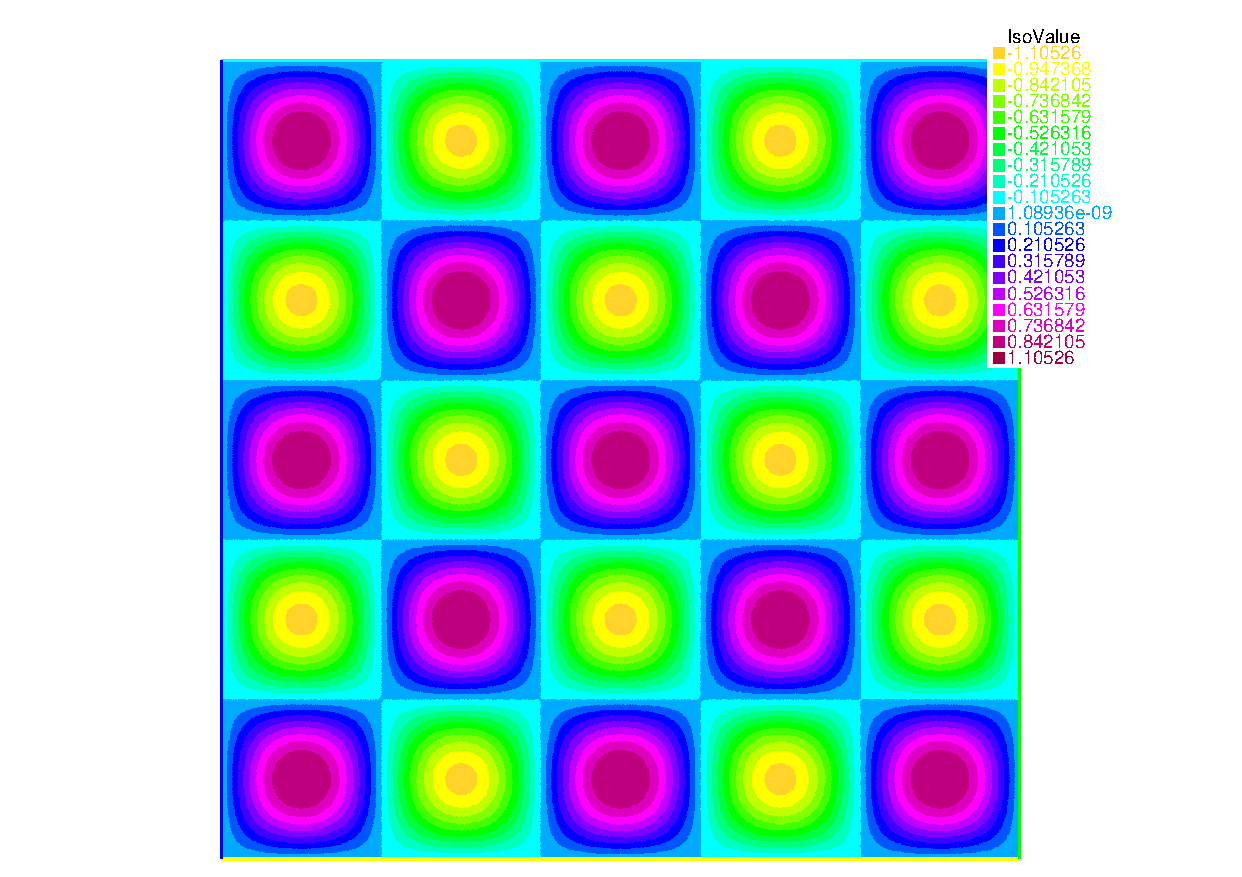
\includegraphics[width=\textwidth]{convergencePk/solution.pdf}
    \captionof{figure}{Exact solution}

    \end{figure}
\end{minipage}
\hspace{0.1cm}
%------------------------------------------
% Colonne de droite
%------------------------------------------
\begin{minipage}[h]{0.50\textwidth}
  \vspace{0.3cm}
    \includegraphics[width=\textwidth]{convergencePk/Poisson_2DC_sanspente.pdf}
\end{minipage}

\end{frame}

%%%%%%%%%%%%%%%%%%%%%%%%%%%%%%%%%%%%%%%%%%%%%%%%%%%%%%%%%%%%%%%%%%%%%%%%%%%%%%%%
\begin{frame}{Conclusion}{}
  %\vspace{2cm}
  \begin{center}
    
  \begin{itemize}[label={},itemsep=2em]
    \item \textcolor{blue}{\Large\textbf{\underline{Conclusion:}}}
    \begin{itemize}[label=$\square$,itemsep=1em]
      \item Analysis of the existing 2D  Lagrange finite elements
      \item Design of a generic 2D $P_k$  element inspired by existing elements
      \item Development of associated quadrature formulas
      \item Online documentation on how to add a FE: https://www.ljll.fr/hecht/ftp/old/freefem/old/manual-full.pdf
    \end{itemize}
    \item \textcolor{blue}{\Large\textbf{\underline{Outlooks:}}}
      \begin{itemize}[label=$\square$,itemsep=1em]
      \item More rigorous verification of convergence
      \item Addressing numerical instability in quadrature formulas
      \item Extension to the case of 3D Lagrange
      \end{itemize}
  \end{itemize}
  \end{center}

\end{frame}

\end{document}